\documentclass[11pt]{article}

\usepackage[a4paper,margin=1in]{geometry}
\usepackage{amsmath,amssymb}
\usepackage{hyperref}
\usepackage{enumitem}
\usepackage{graphicx}
\setlist{nosep}
\hypersetup{
    colorlinks=true,
    linkcolor=blue,
    citecolor=blue,
    urlcolor=blue
}

\title{Context-Dependent Sequential Memory\\in Adaptive Kuramoto Networks}
\author{}
\date{}

\begin{document}

\maketitle

\section{Project Overview}

Associative memory memory models store patterns as stable states, or dynamical attractors, of a system. When the system is initialized with an incomplete, noisy, or slightly distorted version of a stored pattern, its dynamics evolve toward the closest matching memory. In this way, the model retrieves a complete pattern from partial information rather than locating it through an explicit search \cite{hopfield,krotov}.

\begin{figure}[htbp]

    \centering

    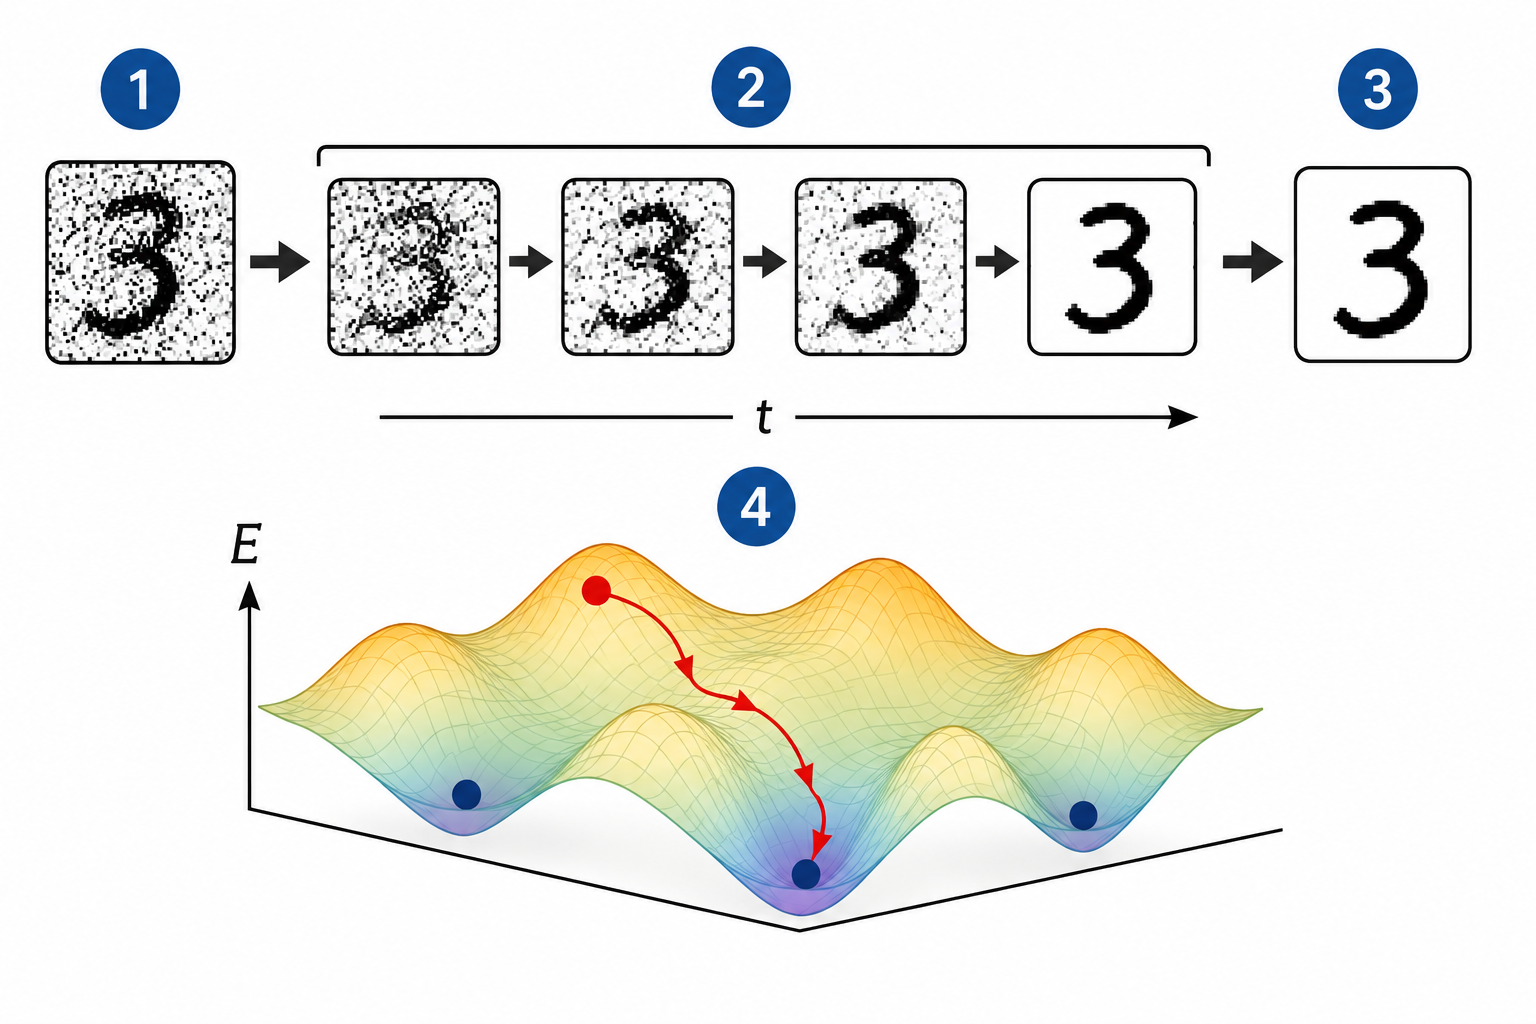
\includegraphics[width=0.75\linewidth]{introduction_visual.png}

    \caption{Associative memory retrieval: (1) a noisy or incomplete cue initializes the system; (2) the state evolves under the network dynamics; (3) the trajectory converges to a stored pattern; and (4) in the energy-landscape interpretation, this evolution corresponds to motion toward a local minimum representing the retrieved memory.}

    \label{fig:associative-memory-retrieval}

\end{figure}

Sequential associative memory extends this idea by storing transitions between patterns \cite{longseq},
\[
A \to B \to C.
\]

A first-order sequential memory models means that the next state depends only on the current state. This project investigates \emph{context-dependent sequential memory}, in which the next state also depends on recently visited states. For example,
\[
(A,B)\to C,
\qquad
(D,B)\to E.
\]
Although both trajectories reach \(B\), their subsequent states differ because their histories differ.

The aim is to develop and study this mechanism in a network of coupled phase oscillators. The project combines nonlinear dynamics, associative memory, numerical simulation, and storage-capacity analysis. The central objective is to determine whether a Kuramoto-type network can reliably select different future states from the same present state using a finite dynamical memory.

\section{Mathematical Framework}

\subsection*{Oscillator dynamics and stored memories}

The classical Kuramoto model is \cite{kuramoto}
\[
\dot{\theta}_i
=
\omega_i
+
\sum_{j=1}^{N}K_{ij}\sin(\theta_j-\theta_i),
\]
where \(\theta_i\in\mathbb{T}\) is the phase of oscillator \(i\), \(\omega_i\) is its natural frequency, and \(K_{ij}\) is the coupling strength.

A memory is represented by a phase configuration
\[
\xi^\mu=(\xi_1^\mu,\ldots,\xi_N^\mu),
\qquad
\mu=1,\ldots,P.
\]
The similarity between the network state and memory \(\mu\) is measured by
\[
m_\mu(t)
=
\frac{1}{N}\sum_{i=1}^{N}
e^{\mathrm{i}(\theta_i(t)-\xi_i^\mu)}.
\]
A value \(\lvert m_\mu\rvert\approx 1\) indicates retrieval of memory \(\mu\).

One possible associative coupling is
\[
J_{ij}
=
\frac{1}{P}
\sum_{\mu=1}^{P}
\cos(\xi_i^\mu-\xi_j^\mu),
\]
giving the memory-stabilizing term
\[
F_i^{\mathrm{mem}}
=
K_1\sum_{j=1}^{N}
J_{ij}\sin(\theta_j-\theta_i).
\]

\subsection*{Finite-memory context}

To retain information about recent states, introduce filtered overlap variables
\[
\tau\dot{h}^{(1)}_\mu
=
-h^{(1)}_\mu+\lvert m_\mu(t)\rvert^2,
\]
\[
\tau\dot{h}^{(r)}_\mu
=
-h^{(r)}_\mu+h^{(r-1)}_\mu,
\qquad r=2,\ldots,M.
\]
The variables \(h_\mu^{(1)},\ldots,h_\mu^{(M)}\) form a delay chain that approximates a context window of length \(M\).

Context-dependent transitions are encoded by a tensor
\[
A_{\mu_1,\ldots,\mu_M}^{\rho},
\]
where a nonzero entry represents the rule
\[
(\mu_1,\ldots,\mu_M)\to\rho.
\]


The proposed oscillator dynamics is
\[
\dot{\theta}_i
=
\omega_i
+
F_i^{\mathrm{mem}}
+
F_i^{\mathrm{tr}},
\]
with
\[
F_i^{\mathrm{tr}}
=
K_T
\sum_{\mu_1,\ldots,\mu_M,\rho}
A_{\mu_1,\ldots,\mu_M}^{\rho}
\left(
\prod_{r=1}^{M}h_{\mu_r}^{(r)}
\right)
\sin(\xi_i^\rho-\theta_i).
\]

The two terms have complementary roles:
\begin{itemize}
    \item \(F_i^{\mathrm{mem}}\) stabilizes the stored phase patterns;
    \item \(F_i^{\mathrm{tr}}\) drives the system toward the next pattern selected by its recent history.
\end{itemize}

This construction can be interpreted as context-dependent dynamical inference rather than full symbolic reasoning. It is closely related to finite-memory Markov models, finite-state automata, sequence prediction, and higher-order associative memory.

\textbf{This is not necessary the final model, with testing and gaining some intuition we can tweak it so that it works}

\section{Research Questions}

The main questions are:

\begin{enumerate}
    \item Can the oscillator network reliably implement branching rules such as
    \[
    (A,B)\to C,
    \qquad
    (D,B)\to E?
    \]

    \item How do retrieval accuracy and storage capacity scale with the number of oscillators \(N\), memories \(P\), stored transitions, and context length \(M\)?

    \item How sensitive is retrieval to phase noise, frequency heterogeneity, imperfect initialization, and interference between sequences?

    \item How do the time scale \(\tau\) and coupling strengths \(K_1\) and \(K_T\) affect stability and transition speed?

    \item What dynamical phenomena arise, including metastability, oscillatory retrieval, spontaneous switching, and synchronization loss?

    \item Can alternative history mechanisms or higher-order interactions improve robustness and capacity?
\end{enumerate}

\section{Project Plan}
\subsection*{0. Reproduce Dense Associative Memory with Higher Order Kuramoto Networks}
(https://arxiv.org/pdf/2507.21984)
Simluate the higher order Kuramoto network and observe DAM


\subsection*{1. Reproduce first-order sequential memory}
(https://arxiv.org/abs/2306.04532v2) 
Begin with an existing implementation of sequential associative memory and study simple trajectories such as
\[
A\to B\to C.
\]
The initial goals are to understand how memories and sequences are generated, how the dynamical equations are integrated, and how successful retrieval is measured.

The primary diagnostic is the overlap matrix
\[
\lvert m_\mu(t)\rvert^2,
\]
visualized as a heatmap over time and memory index. This should distinguish successful transitions, failed retrieval, metastable states, and oscillatory behaviour.

\subsection*{2. Characterize crossing sequences}

Study the first-order system with
\[
A\to B\to C,
\qquad
D\to B\to E.
\]
Because both sequences pass through \(B\), a first-order model cannot explicitly distinguish their histories. Numerical experiments should determine whether one branch dominates, whether the outcome becomes probabilistic, and how interference changes with network size and sequence load.

\subsection*{3. Implement context-dependent retrieval}

Add the history variables \(h_\mu^{(r)}\) and implement the rules
\[
(A,B)\to C,
\qquad
(D,B)\to E.
\]
A minimal test should compare trajectories initialized near \(B\) with different preceding histories and verify that the correct target memory is retrieved.

Relevant measurements include:
\begin{itemize}
    \item target-memory overlap;
    \item transition success rate;
    \item time required for retrieval;
    \item sensitivity to noise and parameter changes;
    \item frequency of incorrect or ambiguous transitions.
\end{itemize}

\subsection*{4. Study scaling and extensions}

Once the basic mechanism is reliable, expand to multiple branching rules and longer contexts. Possible directions include:
\begin{itemize}
    \item empirical storage-capacity scaling;
    \item sparse versus dense transition tensors;
    \item alternative filters or explicit delays;
    \item stability and bifurcation analysis;
    \item mean-field approximations;
    \item metastable or heteroclinic transition structures.
\end{itemize}

\section{Expected Outputs}

The initial project outputs are:

\begin{itemize}
    \item a documented simulation of first-order sequential retrieval;
    \item overlap heatmaps and trajectory visualizations;
    \item a reproducible crossing-sequence experiment;
    \item an implementation of finite-memory context variables;
    \item a demonstration of context-dependent branching;
    \item a brief numerical study of robustness and parameter dependence.
\end{itemize}

Further theoretical analysis can be selected according to the numerical results. The overall outcome should clarify when synchronization-based networks can use recent dynamical history to resolve otherwise ambiguous sequential transitions.

\begin{thebibliography}{9}

\bibitem{kuramoto}
Y.~Kuramoto,
\textit{Chemical Oscillations, Waves, and Turbulence},
Springer Series in Synergetics, vol.~19,
Springer-Verlag, Berlin and Heidelberg, 1984.
\href{https://doi.org/10.1007/978-3-642-69689-3}
{\texttt{doi:10.1007/978-3-642-69689-3}}.

\bibitem{hopfield}
J.~J.~Hopfield,
``Neural networks and physical systems with emergent collective computational abilities,''
\textit{Proceedings of the National Academy of Sciences of the United States of America},
vol.~79, no.~8, pp.~2554--2558, 1982.
\href{https://doi.org/10.1073/pnas.79.8.2554}
{\texttt{doi:10.1073/pnas.79.8.2554}}.

\bibitem{krotov}
D.~Krotov and J.~J.~Hopfield,
``Dense associative memory for pattern recognition,''
in \textit{Advances in Neural Information Processing Systems 29},
D.~D.~Lee, M.~Sugiyama, U.~von Luxburg, I.~Guyon, and R.~Garnett, Eds.,
Curran Associates, Inc., pp.~1172--1180, 2016.
\href{https://proceedings.neurips.cc/paper/2016/hash/eaae339c4d89fc102edd9dbdb6a28915-Abstract.html}
{\texttt{NeurIPS proceedings}}.

\bibitem{longseq}
H.~T.~Chaudhry, J.~A.~Zavatone-Veth, D.~Krotov, and C.~Pehlevan,
``Long sequence Hopfield memory,''
in \textit{Advances in Neural Information Processing Systems 36},
2023.
\href{https://arxiv.org/abs/2306.04532}
{\texttt{arXiv:2306.04532}}.

\end{thebibliography}

\end{document}